\section{Leitungen}
%\includegraphics[width=1\columnwidth]{Figures/ZahlentabelleLeitungsparameter.png}


\subsection{Allgemeine Leitung (mit Verlusten)}
\begin{center}
\resizebox{\columnwidth}{!}{
        \begin{circuitikz}%[american voltages]
            %Schaltbild
            \draw(0,0)
            to[V,v=$u_G(t)$](0,2)                               %Spannungsquelle
            to[R=$Z_g$](3,2)                                    %Quelleninnenwiderstand
            to[short,o-o](7,2)                                  %Leitung mit Knoten
            to[short](8 ,2)
            to[R=$Z_A$](8,0)                                    %Lastwiderstand
            to[short](7,0)                                      
            to[short,o-o](3,0)                                  %Leitung mit Knoten
            to[short](0,0);   

            %Knoten + Leitung Beschreibung
            \draw(3,2) node[above] {Eingang};
            \draw(7,2) node[above] {Ausgang};
            \draw[decoration={brace},decorate]
                 (3,2.6) -- node[above=6pt] {$\underline{Z}_L$} (7,2.6);
            
            %linke gestrichelte linie
            \draw[dotted](3,0)--(3,-0.5) node[left]{$l=-d$};
            \draw[dotted](3,-0.5)--(3,-1) node[left]{$z=d$};
            \draw[dotted](3,-1)--(3,-1.5);

            %Pfeil in richtung l
            \draw[-latex](3,-0.5) -- (7,-0.5);
            \node at (4,-0.5)[above]{positiv $l$};
            
            %rechte gestrichelte Linue
            \draw[dotted](7,0)--(7,-0.5) node[right]{$l=0$};          
            \draw[dotted](7,-0.5)--(7,-1) node[right]{$z=0$};
            \draw[dotted](7,-1)--(7,-1.5);

            %pfeil in richtung z
            \draw[latex-](3,-1) -- (7,-1);
            \node at (6,-1)[above]{positiv $z$};

            %Pfeil in hinlaufende richtung
            \draw[-latex](3,1.25) -- (6.5,1.25);
            \node at (4.5,1.25)[above]{hinlaufende Welle};

            %Pfeil in rücklaufende richtung
            \draw[latex-](3.5,0.5) -- (7,0.5);
            \node at (5.5,0.5)[above]{rücklaufende Welle};
        \end{circuitikz}
}
\end{center}

%Referenzpunkt \textbf{Quelle} ($ z=0 $):
%\begin{align*}
%	\underline{U}(z)   & = \underline{U}_h \cdot e^{-\underline{\gamma}z} + \underline{U}_r \cdot e^{+\underline{\gamma} z}                    \\
%	\underline{I}(z)   & = \underline{I}_h \cdot e^{-\underline{\gamma} z} + \underline{I}_r \cdot e^{+\underline{\gamma} z}
%%	= \frac{U_h}{Z_L}e^{\underline{\gamma} d} - \frac{U_r}{Z_L}e^{-\underline{\gamma} d} 	\\
%\end{align*}
Eingang: $ \underline{Z}_e $ \quad Anfang: $ \underline{Z}(l) = \underline{Z}_1 $ \quad
Abschluss: $ \underline{Z}_2 = \underline{Z}_{(l=0)}$ \\
Referenzpunkt \textbf{Last} ($ l=0 $):
\begin{align*}
	\underline{U}(l)   & = \underline{U}_h \cdot e^{\underline{\gamma}l} + \underline{U}_r \cdot e^{-\underline{\gamma} l}                    \\
	\underline{I}(l)   & = \underline{I}_h \cdot e^{\underline{\gamma} l} + \underline{I}_r \cdot e^{-\underline{\gamma} l}
	%	= \frac{U_h}{Z_L}e^{\underline{\gamma} d} - \frac{U_r}{Z_L}e^{-\underline{\gamma} d} 	\\
\end{align*}

\subsubsection{Gleichungen}
\begin{align*}
	\underline{U}(l)& = \underline{U}_2 \cdot \cosh(\underline{\gamma}l) + Z_L \underline{I}_2 \cdot \sinh(\underline{\gamma}l)\\
	& = \underline{U}_2 \cdot \left[ \cosh(\underline{\gamma} l) + \tfrac{\underline{Z}_L}{\underline{Z}_2} \sinh(\underline{\gamma} l) \right]\\
	\underline{I}(l)& = \underline{I}_2 \cdot \cosh(\underline{\gamma}l) + \frac{\underline{U}_2}{Z_L} \cdot \sinh(\underline{\gamma}l)\\
	& = \underline{I}_2 \cdot \left[ \cosh(\underline{\gamma} l) + \tfrac{\underline{Z}_2}{\underline{Z}_L} \sinh(\underline{\gamma} l) \right]\\
	\underline{Z}(l) & = \frac{\underline{Z}_2+ \underline{Z}_L\tanh(\underline{\gamma} 
		l)}{1+\frac{\underline{Z}_2}{\underline{Z}_L}\tanh(\underline{\gamma} l)} =
		\underline{Z}_L \frac{\underline{Z}_2+ \underline{Z}_L\tanh(\underline{\gamma} 
		l)}{{\underline{Z}_L}+{\underline{Z}_2}\tanh(\underline{\gamma} l)}
\end{align*}
komplexer $\underline{\gamma}$ nicht im TR berechenbar:\\
\underline{Lösung:} $\alpha l \left[ \tfrac{\texttt{Np}}{\texttt{m}} \right] $ und $ \beta l \left[ \tfrac{\texttt{rad}}{\texttt{m}} \right] $ einzeln berechnen, dann:
\begin{align*}
	\cosh(\underline{\gamma}l) &= \frac{1}{2} \left[e^{\alpha l} \cdot e^{j\beta l} + e^{-\alpha l} \cdot e^{-j\beta l} \right]\\
	\sinh (\underline{\gamma}l)&= \frac{1}{2} \left[e^{\alpha l} \cdot e^{j\beta l} - e^{-\alpha l} \cdot e^{-j\beta l} \right]\\
	\tanh(\underline{\gamma}l) &= 
	1+\frac{2}{e^{\alpha l} \cdot e^{j\beta l}-1}
\end{align*}
  $e^{\pm \alpha l }:$ Dämpfung \qquad $e^{\pm j\beta l}:$ Phase ($\angle$ im TR)\\
  Für Winkel $\alpha l$ bzw. $ \beta l$ auf \textbf{RAD} in TR!
\subsubsection{Kenngrößen} 
\begin{itemize}
\item Leitungswellenwiderstand:
\begin{equation*}
    \underline{Z}_L = \sqrt{ \frac{R + j \omega L}{G + j \omega C}} = \frac{\underline{U}_h}{\underline{I}_h} =- \frac{\underline{U}_r}{\underline{I}_r}
\end{equation*}
komplexer $\underline{Z}_L$ nicht in TR berechenbar:\\
\textbf{Betrag}: erst $\underline{Z}_L^2$, dann $\sqrt{|Z_L^2|}$ ermitteln.\\
\textbf{Phase}: $0.5 \cdot \arg(\underline{Z}_L^2)$ \quad
$\rightarrow$  $\underline{\gamma}$ analog vorgehen.

\item Fortpflanzungskonstante:
\begin{align*}
	\underline{\gamma} & = \sqrt{(R+j\omega L)\cdot(G+j\omega C)} = \alpha + j \beta \, \left[ \frac{1}{m} \right]  \\
	& = j \omega \sqrt{LC} \cdot \sqrt{ \frac{RG}{j^2 \omega^2 LC} + \frac{G}{j \omega C} + \frac{R}{j \omega L} + 1}
\end{align*}
\item Reflexionsfaktor: \qquad
$ r(l) \, \widehat{=} \, r_1 $: Leitungs\textit{anfang} 
\begin{align*}
	\underline{r}(l) &= \underline{r}_2 \cdot e^{-2\underline{\gamma}l} = \underline{r}_2\cdot e^{-2\alpha l}\cdot e^{-2j\beta l}\\
	 &= 	\frac{\underline{U}_r(l)}{\underline{U}_h(l)} = -\frac{\underline{I}_r(l)}{\underline{I}_h(l)}
	=\frac{\underline{Z}(l)-\underline{Z}_L}{\underline{Z}(l)+\underline{Z}_L} = \frac{\tfrac{Z(l)}{Z_L}-1}{\tfrac{Z(l)}{Z_L}+1}
\end{align*}
\item weitere Parameter: \qquad meistens $ \mu_r = 1 $
\begin{align*}
    \lambda_0  = \frac{c_0}{f} \qquad \lambda & = \frac{2\pi}{\beta} = \frac{c_0}{f\sqrt{\varepsilon_{r,\texttt{eff}}\cdot \mu_{r,\texttt{eff}}}} \\
    l_{\texttt{elek.}} = \beta \cdot l \qquad v_p & = \frac{\omega}{\beta} = \frac{c_0}{\sqrt{\varepsilon_{r,\texttt{eff}}\cdot \mu_{r,\texttt{eff}}}}
%    \alpha             & = \omega \cdot \sqrt{\dfrac{\mu \varepsilon}{2}\cdot \left(\sqrt{1+\dfrac{\sigma^2}{\omega^2\cdot\varepsilon^2}}{\color{red}{-}}1\right)}           \\
%    \beta              & = \omega \cdot \sqrt{\dfrac{\mu \varepsilon}{2}\cdot \left(\sqrt{1+\dfrac{\sigma^2}{\omega^2\cdot\varepsilon^2}}{\color{green}{+}}1\right)}
\end{align*}
\end{itemize}
\subsubsection{Kurzschluss und Leerlauf}
Eingangswiderstand $ \underline{Z}_e $ am Leitungsende:
\begin{align*}
\text{mit Kurzschluss} \qquad \underline{Z}_{e,\texttt{kurz}} & = \underline{Z}_L \cdot \tanh(\underline{\gamma}l)\\
\text{im Leerlauf} \qquad 
\underline{Z}_{e,\texttt{leer}} & = \tfrac{\underline{Z}_L}{\tanh(\underline{\gamma}l)}\\
\text{beliebige Länge} \qquad \underline{Z}_L &=\sqrt{\underline{Z}_{e,\texttt{kurz}}(l)\cdot \underline{Z}_{e,\texttt{leer}}(l)}
\end{align*}
\subsubsection{Lange und Kurze Leitung}
\begin{itemize}
	\item kurze Leitung $\rightarrow l \ll \tfrac{\lambda}{4} \quad |\underline{\gamma}l| \ll 1 $
		\begin{align*}
			\underline{U}(l) &\approx \underline{U}_2 + \underline{I}_2 \cdot l (R' + jwL')\\
			\underline{I}(l) &\approx \underline{I}_2 + \underline{U}_2 \cdot l (G'+jwC')
		\end{align*}
	Leitung wird durch konzentrierte Elemente ersetzt.
	\item lange Leitung $\rightarrow l \gg \tfrac{\lambda}{4} \quad |\underline{\gamma}l| \gg 1$\\
	Abschluss egal, es wird nur $ \underline{Z}_L = \underline{Z}(l) $ gemessen wird.
\end{itemize}


\subsection{Verlustlose Leitung}
\subsubsection{Kenngrößen}
$ R', G' = 0 \rightarrow \alpha = 0 \qquad Z_L, v_p \nsim f$
\begin{align*}
	Z_L  & =  \sqrt{\frac{L}{C}} \rightarrow \text{rein reell!}                                                                         \\
    \underline{\gamma}  & = j \beta  = j \omega \sqrt{LC} \qquad \beta = \omega \cdot \sqrt{LC} \\
    v_p                & = \frac{\omega}{\beta} = \frac{1}{\sqrt{\mu\varepsilon}}= \frac{c_0}{\sqrt{\mu_r\varepsilon_r}} = \frac{1}{\sqrt{LC}} \\
    \lambda            & = \frac{2\pi}{\beta}= \frac{v_p}{f}= \frac{c_0}{f\sqrt{\mu_r\varepsilon_r}}=\frac{1}{f\sqrt{LC}}
\end{align*}
\subsubsection{verlustloser Reflexionsfaktor}
%$ \underline{U}_r(l) = \underline{U}_r(l=0) \cdot e^{-j\beta l} \qquad \underline{U}_h(l) = \underline{U}_h(l=0) \cdot e^{j\beta l} $

$ \underline{r}_{(l=0)} = \underline{r}_2 \qquad 0<r<1 \qquad 0<\Psi<2\pi $ $\Psi$ in \textbf{RAD}!
\begin{align*}
	\underline{r}(l)  &= \underline{r}_2 \cdot e^{-j2\beta l} = r \cdot e^{-j(\Psi_0+2\beta l)} =r\cdot e^{j\Psi} \\ &=\tfrac{\underline{Z}(l)-Z_L}{\underline{Z}(l)+Z_L}\\
	\underline{r}_2 & = \tfrac{\underline{Z}_2-Z_L}{\underline{Z}_2+Z_L} = \tfrac{\underline{U}_2-\underline{I}_2Z_L}{\underline{U}_2 +\underline{I}_2 Z_L}\\
	\tfrac{\underline{Z}(l)}{Z_L} & = \tfrac{1+\underline{r}(l)}{1-\underline{r}(l)}
\end{align*}
\subsubsection{Beliebiger Abschluss (Last)} \label{beliebig_abschluss}
$\underline{U}_2 = \underline{U}_{(l=0)} =  \underline{U}_h  +\underline{U}_r \qquad \underline{I}_2 = \underline{I}_{(l=0)} =  \underline{I}_h  +\underline{I}_r $	
\begin{align*}
	\underline{Z}(l) & = 
	\frac{\underline{Z}_2+jZ_L\tan(\beta 
	l)}{1+ j \frac{\underline{Z}_2}{Z_L}\tan(\beta l)}
	= Z_L \frac{\underline{Z}_2 + j Z_L \tan(\beta l)}{Z_L + j \underline{Z}_2 \tan(\beta l)}\\
	\underline{U}(l) & = \underline{U}_2 \cdot \left[ \cos(\beta l) + j \tfrac{Z_L}{\underline{Z}_2} \sin(\beta l) \right] \\
	\underline{I}(l) & = \underline{I}_2 \cdot \left[ \cos(\beta l) + j \tfrac{\underline{Z}_2}{Z_L} \sin(\beta l) \right] 
\end{align*}
Für Beträge/Amplitudenwerte: \quad $\left| \frac{\underline{U}}{\underline{U}_2} \right| = \sqrt{\text{Re}^2+\text{Im}^2}  $.\\
Bildung einer Stehenden Welle!
\subsubsection{Kurzschluss an Leitungsende}
$ \underline{Z}_2 = 0 \qquad \underline{U}_2 = \underline{U}_{(l=0)} = 0 \rightarrow \underline{U}_h = - \underline{U}_r \qquad \underline{I}_h = \underline{I}_r $
\begin{align*}
	\underline{Z}(l)         & = \frac{\underline{U}(l)}{\underline{I}(l)} =  Z_L\cdot j\tan(\beta l)        \qquad \rightarrow \text{rein imaginär!}                      \\
	\underline{U}(l) & =  \underline{U}_h  \cdot 2j\sin(\beta l) = \underline{I}_2 Z_L \cdot j\sin(\beta l)\\
	I(l)         & = \underline{I}_h \cdot 2 \cos(\beta l) =\underline{I}_2 \cdot \cos(\beta l) \qquad \underline{I}_2 =\frac{2\underline{U}_h}{Z_L}
%	\hat{U}_E    & = \hat{U}_{generator}\cdot\frac{\underline{Z}_E}{\underline{Z}_{generator}+\underline{Z}_E} \\
\end{align*}
\subsubsection{Leerlauf an Leitungsende}
$ \underline{Z}_2 = \infty \qquad \underline{I}_2 = \underline{I}_{(l=0)} = 0 \rightarrow \underline{I}_h = - \underline{I}_r \qquad \underline{U}_h = \underline{U}_r $
\begin{align*}
	\underline{Z}(l) & = \frac{\underline{U}(l)}{\underline{I}(l)}  = -j \,\frac{Z_L}{\tan(\beta l)}\qquad\rightarrow \text{rein imaginär!}                 \\
		\underline{U}(l) & = \underline{U}_h \cdot 2 \cos(\beta l) = \underline{U}_2 \cdot \cos(\beta l) \qquad \underline{U}_2 = 2\underline{U}_h\\
	\underline{I}(l)         & = \underline{I}_h\cdot 2j\sin(\beta l) = \frac{\underline{U}_2}{Z_L} \cdot  j \sin(\beta l)
%	r_A          & = 1                                                                              \\
%	\mathrm{SWR} & = \infty                                                                         \\
\end{align*}

\subsubsection{Leitung als Impedanz-Transformator}
$\lambda / 4$ -Leitung mit Eingangswiderstand $ \underline{Z}_e = \underline{Z}(l) $ aus  \ref{beliebig_abschluss}:
\begin{align*}
	\frac{\underline{Z}_e}{Z_L} & = \frac{Z_L}{\underline{Z}_2} = \frac{\underline{Y}_2}{Y_L} \rightarrow Z_e = \frac{Z^2_L}{\underline{Z}_2}
\end{align*}
Eine $ \lambda / 4 $ -Leitung transformiert:
L $ \leftrightarrow $ C, \\Kurzschluss $ \leftrightarrow $ Leerlauf, \textbf{großes} R $ \leftrightarrow$ \textbf{kleines} R

%\subsubsection{vernachlässigbarer Widerstandsbelag}
%\includegraphics[width=\columnwidth]{Figures/vernachlaessigbarerWiderstandsbelag.png}
%
%
%\subsubsection{vernachlässigbarer Leitwertbelag}
%\includegraphics[width=\columnwidth]{Figures/vernachlaessigbarerLeiterwertbelag.png}

\subsubsection{Angepasste (reflexionsfreie) Leitung}
Eingangswiderstand $ Z_1\nsim$ Leitungslänge, rein reell!\\
Nur hinlaufende Welle, \textbf{reflexionsfrei}!
\begin{align*}
	Z_L          & = Z_1 = Z_2 = Z(l) \qquad
	r_A          =0 \qquad 
	\mathrm{SWR} = 1  \\
	U(z)         & = U_h\cdot e ^{j\beta z}  \qquad           
	I(z)         = I_h \cdot e^{j\beta z} = \frac{U_h}{Z_L}\cdot e^{j\beta z}
\end{align*}

\subsubsection{Ohmscher Abschluss an Leitungsende}
$ r_2 \rightarrow$ rein reell! 
\begin{align*}
	R_A > Z_L & \rightarrow\theta_r = 0 \rightarrow r_A \texttt{ ist negativ} \\
	& \rightarrow z_\texttt{max}=\frac{\lambda}{2}\cdot n\\
	R_A < Z_L& \rightarrow\theta_r = \pi                           \\
	& \rightarrow z_\texttt{min}=\frac{\lambda}{2}\cdot n
\end{align*}

\subsubsection{Position von Extrema}
bei beliebigen Abschlüssen/Lasten! $ \rightarrow $ stehende Welle!
\begin{gather*}
	\boxed{r_A = |r_A|\cdot e^{-j\Psi_r}}\rightarrow\Psi_r\text{ in rad}\\
	f_\texttt{min}\rightarrow \text{Minimum(Knoten) der Spannungen}\\
	f_\texttt{max}\rightarrow \text{Maximum(Bäuche) der Spannungen}
\end{gather*}
\begin{align*}
	\lambda_\texttt{min/max} & = \frac{c_0}{f_\texttt{min/max}\sqrt{\mu_{r1}\varepsilon_{r1}}}                                                                                                 \\
	z_\texttt{min}           & =\frac{-n\cdot\lambda_\texttt{min}}{2}                                        \qquad\rightarrow n = -\frac{2z}{\lambda_\texttt{min}}                            \\
	z_\texttt{max}           & =\frac{-(2n+1)\lambda_\texttt{max}}{4}                                        \qquad\rightarrow n = -\frac{4z+\lambda_\texttt{max}}{2\cdot\lambda_\texttt{max}} \\
	z                        & = \frac{\lambda_\texttt{min}\cdot\lambda_\texttt{max}}{4(\lambda_\texttt{min}-\lambda_\texttt{max})}
\end{align*}

\subsubsection{Vorgehen Eingangswiderstand}
Wenn mit Smithdiagramm gearbeitet wird liefert dieses Schritte \ref{Ref L_anfang} und \ref{Bestimmen Z_E}
\begin{enumerate}
    \item Lastimpedanz
          \[ \underline{Z}_A = \dfrac{1}{\frac{1}{R_A} + j \omega C_A} \]
    \item Reflexion am Leitungsende
          \[ \underline{r}_A = \underline{r}(z=0) = \dfrac{Z_A - \underline{Z}_L}{Z_A + \underline{Z}_L} \]
    \item Reflexion am Leitungsanfang \label{Ref L_anfang}
          \[ \underline{r}_E = \underline{r}(z=d) =  \underline{r}_A \cdot e^{-j 2 \beta d}\]
    \item Bestimmung der Impedanz \label{Bestimmen Z_E}
          \[ \underline{Z}_E = \underline{Z}_L \cdot \dfrac{1 + \underline{r}_E}{1 - \underline{r}_E}\]
    \item Eingangswiderstand
          \[ \underline{Z}_E = \dfrac{1}{\frac{1}{\underline{Z}_E} + j \omega C_E}\]
\end{enumerate}

%\subsubsection{Reflexionsfaktor entlang einer Leitung}
%\begin{align*}
%    r_E    & = r_A  ^{-2\underline{\gamma} l} = r_A  e^{-2\alpha l} e^{-j2\beta l}                                                     \\
%    \alpha & = -\frac{\ln(r_A)}{2l} [\si{Np/m}]                                    & \beta & = \dfrac{\phi_2 -\phi_1}{2l} [\si{rad/m}]
%\end{align*}

\subsubsection{Stehwellenverhältnis (SWR)}
Smith-Chart: Kap. \ref{sec:Smith_All} \qquad VSWR: Kap. \ref{sec:VSWR}
\begin{align*}
    &s = \mathrm{SWR}       = \frac{U_\text{max}}{U_\text{min}} = \frac{I_\text{max}}{I_\text{min}} = \frac{1+|r(l)|}{1-|r(l)|} = \frac{|U_h|+|U_r|}{|U_h|-|U_r|}= \dfrac{R_{\text{max}}}{Z_L}&                                                        \\
    &m = \mathrm{SWR}^{-1} = \dfrac{R_{\text{min}}}{Z_L} \qquad |r_2| = \frac{\text{SWR}-1}{\text{SWR}+1} = \frac{1-m}{1+m} &
\end{align*}

\subsubsection{Leistung}
\begin{align*}
    P_{A}            & = P_{H}-P_{R}                                                                                                
                     \quad = \frac{1}{2} \cdot \frac{\hat{U}_{h}^{2}}{Re\{Z_{L}\}}-\frac{1}{2} \cdot \frac{\hat{U}_{r}^{2}}{Re\{Z_{L}\}} \\
                     & =\frac{1}{2} \cdot \frac{\hat{U}_{h}^{2}}{Re\{Z_{L}\}} \cdot\left(1-r^{2}\right)                              \\
                     & = P_{\max} \cdot\left(1-r^{2}\right)                                                                          \\
                     & = \underline{U}_A\cdot\underline{I}_A^*                                                                       \\
    P_V              & = P_q -P_A                                                                                                    \\
    \underline{I}(z) & = \hat{I}\cdot e^{-\alpha z}\angle \beta z
	\end{align*}
\subsubsection{Gleichspannungswert (=Endwert)}
\begin{align*}
    U_A & = U_q\cdot\frac{R_A}{R_i+R_A}
\end{align*}






%\subsubsection{Ohmscher Abschluss an Leitungsende}
%$ r_2 \rightarrow$ rein reell! 
%\begin{align*}
%    R_A > Z_L & \rightarrow\theta_r = 0 \rightarrow r_A \texttt{ ist negativ} \\
%                          & \rightarrow z_\texttt{max}=\frac{\lambda}{2}\cdot n\\
%    R_A < Z_L& \rightarrow\theta_r = \pi                           \\
%                          & \rightarrow z_\texttt{min}=\frac{\lambda}{2}\cdot n
%\end{align*}

\subsection{Mehrfachreflexionen bei fehlender Anpassung}
\begin{center}
    \begin{tikzpicture}
        %Linien
        \draw[-Latex] (1,1) -- (1,0) node [below] {$t$};
        \draw[-,line width=1pt] (1,1) -- (1,6);
        \draw[-,line width=1pt] (5,0) -- (5,6);

        %Pfeile mit Bezeichnungen
        \draw[-Latex] (3.5,6.5) -- (5,6.5)node[right]{$z$};

        \draw[-Latex] (1,6) -- (5,5) node[right]{$t_d$} node[midway, above]{$u_{1h}$};
        %\draw[-] (1,6) -- (3,5.5) node[above]{$U_{1h}$};

        \draw[-Latex] (5,5) -- (1,4)node[left]{$2\cdot t_d$} node[midway, above]{$u_{1r}$};
        %\draw[-] (5,5) -- (3,4.5) node[above]{$U_{1r}$};

        \draw[-Latex] (1,4) -- (5,3)node[right]{$3\cdot t_d$} node[midway, above]{$u_{2h}$};
        %\draw[-] (1,4) -- (3,3.5) node[above]{$U_{2h}$};

        \draw[-Latex] (5,3) -- (1,2)node[left]{$4\cdot t_d$} node[midway, above]{$u_{2r}$};
        %\draw[-] (5,3) -- (3,2.5) node[above]{$U_{2r}$};

        \draw[-Latex] (1,2) -- (5,1)node[right]{$5\cdot t_d$} node[midway, above]{$u_{3h}$};
        %\draw[-] (1,2) -- (3,1.5) node[above]{$U_{3h}$};


        \draw[dotted ] (5,1) -- (3,0.5);

        %Klammern mit Bezeichnungen
        \draw [black,
            decorate,
            decoration = {brace,
                    raise=5pt,
                    amplitude=5pt}] (5,5.8) --  (5,5.2);
        \node at (5.5,5.5)[right]{$u_A = 0$};

        \draw [black,
            decorate,
            decoration = {brace,
                    raise=5pt,
                    amplitude=5pt}] (1,4.2) --  (1,5.8);
        \node at(0.5,5)[left]{$u_E = u_{1h}$};

        \draw [black,
            decorate,
            decoration = {brace,
                    raise=5pt,
                    amplitude=5pt}] (5,4.8) --  (5,3.2);
        \node at (5.5,4)[right]{$u_A = u_{1h}(1+\underline{r}_A)$};

        \draw [black,
            decorate,
            decoration = {brace,
                    raise=5pt,
                    amplitude=5pt}] (1,2.2) --  (1,3.8);
        \node at (0.5,3)[left]{$u_E = u_{1h}$};
        \node at (0.5,2.5)[left]{$+(1+\underline{r}_I)u_{1r}$};

        \draw [black,
            decorate,
            decoration = {brace,
                    raise=5pt,
                    amplitude=5pt}] (5,2.8) --  (5,1.2);
        \node at (5.5,2)[right]{$u_A = u_{1h}(1+\underline{r}_A)$};
        \node at (5.5,1.5)[right]{$+u_{2h}(1+\underline{r}_A)$};


        \draw [black,
            decorate,
            decoration = {brace,
                    raise=5pt,
                    amplitude=5pt}] (1,0.2) --  (1,1.8);
        \node at (0.5,1.5)[left]{$u_E = u_{1h}$};
        \node at (0.5,1)[left]{$+(1+\underline{r}_I)u_{1r}$};
        \node at (0.5,0.5)[left]{$+(1+\underline{r}_I)u_{2r}$};
    \end{tikzpicture}
\end{center}

\begin{align*}
    %u_{1h} & = u_G\cdot\frac{ Z_L}{R_I + Z_L}            \\
    u_{1r} & = r_A\cdot u_{1h}                                \\
    u_{2h} & = r_I\cdot u_{1r} = r_I\cdot r_A\cdot u_{1h}     \\
    u_{2r} & = r_A\cdot u_{2h} = r_I\cdot r_A^2\cdot u_{1h}   \\
    u_{3h} & = r_I\cdot u_{2r} = r_I^2\cdot r_A^2\cdot u_{1h}
\end{align*}
\begin{center}
    \resizebox{\columnwidth}{!}{
        \begin{circuitikz}
            \draw(0,0)
            to[V,v=$u_G(t)$](0,2)                               %Spannungsquelle
            to[R=$R_I \neq Z_L$](2,2)                           %Quelleninnenwiderstand
            to[TL, o-o](5,2)                                    %Leitung oben
            to[short](7,2)
            to[R=$R_A \neq Z_L$](7,0)                           %Quelleninnenwiderstand
            to[short](5,0)
            (2,0) to [TL, o-o](5,0)                             %Leitung unten
            (2,0) to [short](0,0)
            (2,2) to [open, v=$u_E(t)$] (2,0)                   %Spannungspfeil u_E(t)
            (3.5,2) to [open, v=$u(z\mathpunct{,}t)$] (3.5,0)   %Spannungspfeil u(z,t)
            (5,2) to [open, v=$u_A(t)$] (5,0);                  %Spannungspfeil u_A(t)
            \draw[dotted] (2,2) -- (2,2.5);
            \draw[dotted] (5,2) -- (5,2.5);
            \draw[Latex-Latex, yshift=3ex] (2,2) -- (5,2);
            \node at (3.5,2) [above, yshift=3.5ex] {$l_e$};
            \node at (3.5,0) [below, yshift=-1.4ex] {$Z_L\mathpunct{,}c$};
        \end{circuitikz}
    }
\end{center}

\begin{align*}
     & \text{Reflexionsfaktor Leitungsanfang: } & \underline{r}_I & = \frac{R_I - Z_L}{R_I + Z_L}                 \\
     & \text{Reflexionsfaktor Leitungsende: }   & \underline{r}_A & = \frac{R_A - Z_L}{R_A + Z_L}                 \\
     & \text{Hinlaufende Welle}                 & u_{1h}          & = \hat{u}_G \cdot\frac{Z_L}{Z_L+R_I}          \\
     & \text{Signallaufzeit: }                  & t_d             & = \frac{l}{c_0}\cdot\sqrt{\mu_r\varepsilon_r} \\
     &                                          &                 & = \frac{l}{v_p}
\end{align*}
%\subsection{Kettenmatrix einer Leitung}
%\[
%    A =
%    \left[ {\begin{array}{cc}
%                    \cosh(\gamma l)               & Z_L \sinh(\gamma l) \\
%                    \frac{1}{Z_L} \sinh(\gamma l) & \cosh(\gamma l)     \\
%                \end{array} } \right]
%\]
\subsection{Leitungsparameter}
				\subsubsection{Allgemein}
Für beliebige Leitergeometrie gelten folgende Zusammenhänge:
\[
\boxed{LC = \mu\varepsilon} \quad \text{und} \quad \boxed{\frac{G}{C} = \frac{\sigma}{\varepsilon}}
\]
Innere Induktivität:
\[
L_i = \frac{R}{w}
\]
\textbf{\color{red}{Leitungen gehen HIN und ZURÜCK!!!}\\
	\color{red}{Länge verdoppeln!!!}
}
\subsubsection{Streifenleitung / Parallele Platten}
Für Sinus-Anregung:
\begin{align*}
	I(l) & = \frac{U}{Z_L} = \underbrace{\frac{U_0}{Z_L}}_{I_0}\cdot e^{-j\beta l\cdot e^{j\omega t}}                         \\
	U(l) & = \int \vec{E} d\vec{s} \stackrel{b\gg d}{=} E\cdot d \rightarrow  &E = \frac{U_0}{d}\cdot^{-j\beta l}\cdot\vec{e}_x \\
	I(l) & = \oint \vec{H} d\vec{s} =  H\cdot b \rightarrow &H = \frac{I_0}{b}\cdot^{-j\beta l}\cdot\vec{e}_y                  % \\
	% \vec{E}(r, z) & = \frac{I}{2\pi r}\cdot Z_F\cdot e^{-j\beta z} \cdot\vec{e}_r                                                      \\
	%               & = \frac{\hat{U}}{r \cdot\ln{(^{2b}/_{2a})}}\cdot e^{-j\beta z}\cdot\vec{e}_r
\end{align*}
$ \mathbf{b} $: Platten\textbf{breite} \qquad $ \mathbf{d} $: Abstand zwischen den Platten\\

\begin{minipage}[t]{0.4\columnwidth}
	\begin{tikzpicture}
    \tikzset{cross/.style={cross out, draw=black, minimum size=2*(#1-\pgflinewidth), inner sep=0pt, outer sep=0pt},
        %     %default radius will be 1pt. 
        cross/.default={3.5pt}}

        %Untereplatte
        \draw[-](0,0)--(0,0.35);
        \draw[-](2,0)--(2,0.35);

        \draw[-](0,0)--(2,0);
        \draw[-](0,0.35)--(2,0.35);

        \draw[-](0,0.35)--(0.3,0.65);
        \draw[-](2,0)--(3,1);
        \draw[-](2,0.35)--(3,1.35);

        \draw[-](1,0.175) circle (0.15);
        \draw[-,fill=black!100] (1,0.175) circle (0.05);

        %Obere Platte
        \draw[-](0,0.65)--(0,1);
        \draw[-](2,0.65)--(2,1);

        \draw[-](0,0.65)--(2,0.65);
        \draw[-](0,1)--(2,1);

        \draw[-](0,1)--(1,2);
        \draw[-](2,1)--(3,2);
        \draw[-](2,0.65)--(3,1.65);

        \draw[-](1,0.825) circle (0.15);
        \draw(1,0.825) node [cross] {};
   
\end{tikzpicture}

\end{minipage}
\begin{minipage}[b][1cm]{0.6\columnwidth}
	\begin{flalign*}
		&R'=\frac{2}{\delta\kappa b}\left[ \frac{\Omega}{m} \right] & &L'=\frac{\mu d}{b} \left[\frac{H}{m}\right]&\\
		&G'=\frac{\kappa b}{d} \left[ \frac{S}{m} \right] &
		&C'=\frac{b\varepsilon}{d} \left[\frac{F}{m}\right]
	\end{flalign*}
\end{minipage}
%
%
%{\renewcommand*{\arraystretch}{0.2}
	%	\begin{tabularx}{0.5\columnwidth}{X}
		%		\hline
		%		\[R'=\frac{2}{\delta\kappa b}\] \\
		%		\hline
		%		\[L'=\frac{\mu d}{b}\]         \\
		%		\hline
		%		\[G'=\frac{\sigma b}{d}\]      \\
		%		\hline
		%		\[C'=\frac{b\varepsilon}{d}\]  \\
		%		\hline
		%	\end{tabularx}
	%}

\subsubsection{Doppelleitung}
$ \kappa $: Leitwert des Dielektrikums \qquad $ \kappa_L $ Leitwert des Leiters\\
$ \mathbf{r} $: Leiterradius \qquad $ \mathbf{d} $: Abstand zw. Leitermitten

\begin{minipage}[t]{0.4\columnwidth}
	\begin{tikzpicture}
    \tikzset{cross/.style={cross out, draw=black, minimum size=2*(#1-\pgflinewidth), inner sep=0pt, outer sep=0pt},
        %     %default radius will be 1pt. 
        cross/.default={3.5pt}}

        %linker Außenleiter
        \draw[-](-0.53,0.53)--(0.97,2.03);

        
        \draw[-](48:0.75) arc (48:312:0.75);

        %linker Innenleiter
        \draw[dashed](-0.106,0.106)--(0.41,0.622);
        \draw[dashed](0.106,-0.106)--(0.922,0.71);

        \draw[-](0,0) circle (0.15);
        \draw(0,0) node [cross] {};


        
        %%%%%%%%%%%%%%%%%%%%%%%%%%%%%%%%%%%%%%%%%%%%%%%%%%%%%%%%%%%
        %%%%%%%%%%%%%%%%%%%%%%%%%%%%%%%%%%%%%%%%%%%%%%%%%%%%%%%%%%%

        %Rechter Außenleiter
        \draw[-](0.48,0.58)--(1.97,2.03);
        \draw[-](1.53,-0.53)--(2.13,0.07);
        \draw([shift={(228:0.75)}]1,0) arc (-132:132:0.75);

        %Rechter Innenleiter
        \draw[dashed](0.894,0.106)--(1.41,0.622);
        \draw[dashed](1.106,-0.106)--(1.622,0.41);

        \draw[-](1,0) circle (0.15);
        \draw[-,fill=black!100] (1,0) circle (0.05);

        

\end{tikzpicture}

\end{minipage}
\begin{minipage}[b][4cm]{0.6\columnwidth}
	\begin{flalign*}
		&R'=\frac{1}{\pi a\delta\kappa_L} \left[ \frac{\Omega}{m} \right] &\\
		&L'= \frac{\mu}{\pi} \cosh^{-1}\frac{d}{2r} \left[\frac{H}{m}\right]&\\
		&G'= \frac{\pi\kappa}{\cosh^{-1}(^d/_{2r})} \left[ \frac{S}{m} \right] &\\
		&C'=\frac{\pi\varepsilon}{\cosh^{-1}(^d/_{2r})} \left[\frac{F}{m}\right]
	\end{flalign*}
\end{minipage}

%{\small\[
	%	\text{cosh am TR: MENU $\rightarrow$ 1; OPTN $\rightarrow$ 1 $\rightarrow$ 5}\\
	%	\]}
%\begin{tikzpicture}
    \tikzset{cross/.style={cross out, draw=black, minimum size=2*(#1-\pgflinewidth), inner sep=0pt, outer sep=0pt},
        %     %default radius will be 1pt. 
        cross/.default={3.5pt}}

        %linker Außenleiter
        \draw[-](-0.53,0.53)--(0.97,2.03);

        
        \draw[-](48:0.75) arc (48:312:0.75);

        %linker Innenleiter
        \draw[dashed](-0.106,0.106)--(0.41,0.622);
        \draw[dashed](0.106,-0.106)--(0.922,0.71);

        \draw[-](0,0) circle (0.15);
        \draw(0,0) node [cross] {};


        
        %%%%%%%%%%%%%%%%%%%%%%%%%%%%%%%%%%%%%%%%%%%%%%%%%%%%%%%%%%%
        %%%%%%%%%%%%%%%%%%%%%%%%%%%%%%%%%%%%%%%%%%%%%%%%%%%%%%%%%%%

        %Rechter Außenleiter
        \draw[-](0.48,0.58)--(1.97,2.03);
        \draw[-](1.53,-0.53)--(2.13,0.07);
        \draw([shift={(228:0.75)}]1,0) arc (-132:132:0.75);

        %Rechter Innenleiter
        \draw[dashed](0.894,0.106)--(1.41,0.622);
        \draw[dashed](1.106,-0.106)--(1.622,0.41);

        \draw[-](1,0) circle (0.15);
        \draw[-,fill=black!100] (1,0) circle (0.05);

        

\end{tikzpicture}

%{\renewcommand*{\arraystretch}{0.2}
	%	\begin{tabularx}{0.5\columnwidth}{|X|}
		%		\hline
		%		\[R  = \frac{1}{\pi a\delta\sigma_c}\]              \\
		%		\hline
		%		\[L = \frac{\mu}{\pi} \cosh^{-1}\frac{d}{2a}\]      \\
		%		\hline
		%		\[G = \frac{\pi\sigma}{\cosh^{-1}(^d/_{2a})}\]      \\
		%		\hline
		%		\[C = \frac{\pi\varepsilon}{\cosh^{-1}(^d/_{2a})}\] \\
		%		\hline
		%\end{tabularx}}
		
		\subsubsection{Koaxialleitung}
		%{\small\[
			%	a = \text{innen Radius} \qquad b = \text{außen Radius} \\
			%	\]}
		Mit Hin- und Rückleiter.
		$ r_i $: Innenradius \quad $ r_a $: Außenradius
		\begin{align*}
			\vec{H}(r, z)         & = \frac{\hat{I}}{2\pi r}\cdot e^{-j\beta z}\cdot\vec{e}_\varphi                   \\
			\vec{E}(r, z)         & = \frac{\hat{I}}{2\pi r}\cdot Z_{F0}\cdot e^{-j\beta z} \cdot\vec{e}_r
			= \frac{\hat{U}}{r \cdot\ln{(^{r_a}/_{r_i})}}\cdot e^{-j\beta z}\cdot\vec{e}_r        \\
			S_{av} & = \frac{1}{2}\cdot\left( \frac{\hat{I}}{2\pi r}\right)^2\cdot Z_{F0}\\
   			Z_L &= \frac{Z_{F0}}{2\pi}\sqrt{\frac{\mu_r}{\varepsilon_r}}\ln\left( \frac{r_a}{r_i} \right)  =\frac{60\Omega}{\sqrt{\varepsilon_r}}\cdot \ln{\frac{r_a}{r_i}}
		\end{align*}
		\begin{minipage}[c][2cm]{0.4\columnwidth}
			%	\begin{tikzpicture}
    \tikzset{cross/.style={cross out, draw=black, minimum size=2*(#1-\pgflinewidth), inner sep=0pt, outer sep=0pt},
        %     %default radius will be 1pt. 
        cross/.default={3.5pt}}

        %Außenleiter
        \draw[-](-0.53,0.53)--(1.07,2.13);
        \draw[-](0.53,-0.53)--(2.23,1.17);

        \draw[-](0,0) circle (0.75);

        %Innenleiter
        \draw[-](-0.106,0.106)--(0.41,0.622);
        \draw[-](0.106,-0.106)--(0.622,0.41);

        \draw[-](0,0) circle (0.15);
        \draw(0,0) node [cross] {};

\end{tikzpicture}

			\begin{center}
    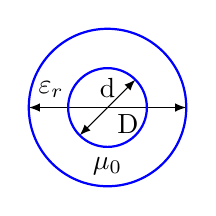
\begin{tikzpicture}
        \draw[latex-latex](-1,0)node[above right]{$\varepsilon_r$}--(1,0);
        \node[below right, yshift=1pt]{D};
        \draw[latex-latex, rotate=45](-0.5,0)--(.5,0);
        \node at (0,0)[above]{d};
        \draw[-, thick, blue](0,0) circle (1);
        \node at(0,-.75)[]{$\mu_0$};
        \draw[-, thick, blue](0,0) circle (0.5) ;
    \end{tikzpicture}


    D = Außendurchmesser

    d = Innendurchmesser
\end{center}
\vspace{-1em}

		\end{minipage}
		\begin{minipage}[c][4cm]{0.6\columnwidth}
			\begin{flalign*}
				&R'=\frac{1}{2\pi\delta\kappa_L}\left(\frac{1}{r_a}+\frac{1}{r_i}\right) \left[ \frac{\Omega}{m} \right] &\\
				&L'=\frac{\mu_0\mu_r}{2\pi}\ln\frac{r_a}{r_i} \left[\frac{H}{m}\right]&\\
				&G'=\frac{2\pi\kappa}{\ln(r_a/r_i)} \left[ \frac{S}{m} \right] &\\
				&C'=\frac{2\pi\varepsilon_0 \varepsilon_r}{\ln(r_a/r_i)} \left[\frac{F}{m}\right]\\
			\end{flalign*}
		\end{minipage}
%	\vspace{5pt}
\\
\\
	\textbf{Dielektrische Dämpfungsverluste}: für sehr hohe $ f $\\
	$G\ll\omega C$, \quad $\tan\delta= (G/\omega C) <0,1$
	\[
	\alpha_d = \frac{\sqrt{\varepsilon_r}\pi f}{c_0}\cdot\tan\delta \sim f
	\]
	
		%
		%
		%{\renewcommand*{\arraystretch}{0.2}
			%	\begin{tabularx}{0.5\columnwidth}{|X|}
				%		\hline
				%		\[R=\frac{1}{2\pi\delta\sigma_c}\left[\frac{1}{a}+\frac{1}{b}\right]\] \\
				%		\hline
				%		\[L=\frac{\mu}{2\pi}\ln\frac{b}{a}\]                                   \\
				%		\hline
				%		\[G=\frac{2\pi\sigma}{\ln(^b/_a)}\]                                    \\
				%		\hline
				%		\[C=\frac{2\pi\varepsilon}{\ln(^b/_a)}\]                               \\
				%		\hline
				%\end{tabularx}}
%				\vspace{1ex}

